\chapter{Introducción}
\pagenumbering{arabic}
\setcounter{page}{1}
%\renewcommand{\baselinestretch}{2} %doble espacio paratodo el texto
En el siguiente capítulo presentamos las razones que nos motivaron al desarrollo de la presente tesis, además el planteamiento del problema principal y como se puede resolver, los objetivos que realizamos, la importancia de realizar la presente, la contribución que realizamos y por último la estructura detallada por capítulos de la presente.

\vskip 0.3cm  

\section{Motivación}

En la actualidad, la sociedad considera de mucha importancia contar con sistemas basados el reconocimiento de expresiones faciales en secuencia de imágenes en diferentes aspectos de nuestra vida diaria, por esto se ha convertido en un reto de la tecnología contemporánea debido a las inmensas aplicaciones que abarca el tema y a la sofisticada que es su técnica, ya que las aplicaciones desarrolladas no son muy eficientes y eficaces debido a la gran variedad de características del rostro y a las condiciones del medio.
\vskip 0.3cm
Por lo tanto, se puede concluir usar secuencia dinámica de imágenes como medio de almacenamiento, esto nos brindaría más datos que ayudarían a un mejor reconocimiento.


\section{Formulación del problema}

  En este trabajo, se propone diseñar un agente inteligente para responder a la siguiente pregunta:
 \begin{center} 
     ?`Cómo reconocer expresiones faciales en secuencias dinámicas de imágenes?
 \end{center}

\section{Importancia de la investigación} 

{\bf Ejemplo:}\par
% ejemplo de tabla

\begin{center}
\begin{table}[ht!]
\centering
\caption{Estimativa en los programas de colecta selectiva formal (2008)}
\begin{tabular}{llr} \toprule
Residuos & Residuos colectados(t/día) & Residuos reciclados(t/año) \\ \midrule
Metales & 5 293 & 9 817 \\
Papeles & 23 997 & 3 827 \\
Plástico & 24 847 & 962 \\
Vidrio & 4 388 & 489 \\ \bottomrule
\end{tabular}
\vskip 0.2cm
\begin{center}
{\small{Fuente: \cite{MMA}.}}
\end{center}
\end{table}
\end{center}
\vskip 0.5cm


%\begin{table}[ht!]
%\centering
%\caption{Estimativa en los programas de colecta selectiva formal (2008)}
%\begin{tabular}{|c|c|c|c|}  \hline 
%Residuos & Residuos colectados(t/día) & Residuos reciclados(t/año) \\ \hline 
%Metales & 5 293 & 9 817 \\
%Papeles & 23 997 & 3 827 \\ 
%Plástico & 24 847 & 962 \\
%Vidrio & 4 388 & 489  \\\hline
%\end{tabular}
%\begin{center}
%{\small{Fuente: \cite{MMA}.}}
%\end{center}
%\end{table}

\section{Objetivos}
A continuación presentamos los objetivos que aspiramos alcanzar con el desarrollo de esta tesis:

\subsection{General}
\begin{enumerate}
\item[•] Diseñar un agente inteligente que permita reconocer expresiones faciales en secuencias dinámicas de imágenes.
\end{enumerate}
\vskip 0.3cm


\subsection{Específicos}

\begin{enumerate}
\item[a)] Desarrollar un agente inteligente con un nivel de sensibilidad mayor o igual a 90%.
\item[b)] Procurar un nivel de especificidad mayor 95%.
\item[c)] Obtener una tasa de reconocimiento de expresiones faciales mayor o igual al 90%.
\item[d)] Determinar los resultados de aplicar el reconocimiento del agente a un conjunto de
expresiones faciales seleccionadas.
\end{enumerate}

\section{Contribución de la investigación}

El trabajo a desarrollar aporta al área computación ya que pretende investigar nuevas técnicas
en procesamiento de imágenes y en procesamiento de secuencia de imágenes que puedan
ser aplicadas a distintas áreas o actividades como seguridad, control, etc.
\vskip 0.3cm
El presente trabajo academicamente permite poner en practica los conocimientos adquiridos
durante nuestra formación académica y profesional permitiéndonos validar y aportar a la
solución de problemas con lo aprendido en materias de la carrera. 

\section{Método de la investigación}
De acuerdo con \cite{Erica}, para el desarrollo del método debe presentarse un bosquejo de la manera  en que se propone llevar a cabo la investigación, es decir, el camino a seguir o los pasos a seguir para realizar una cosa. Cuando mas complejo sea el bosquejo  más fácil se desarrollará el proceso de investigación. Se utiliza el vocablo método en vez de metodología, ya este último se considera equivocado, en el sentido en que se le utiliza comúnmente en informes de investigación. 
\vskip 0.3cm
Los tipos de método a usar para TG en informática se considera:
\begin{enumerate}
\item[a)] {\bf Método deductivo:} Es un método de razonamiento que consiste en tomar conclusiones generales para explicaciones partículares. El método se inicia con el análisis de los postulados, teoremas, leyes, principios, etc., de aplicación universal y de comprobada validez, para aplicarlos  a soluciones o hechos particulares. 

\item[b)]{\bf Método cuantitativo:} Se fundamenta en la medición de las características de los fenómenos, lo cual supone derivar de un marco conceptual pertinente al problema analizado, una serie de postulados que expresen relaciones entre las variables estudiadas de forma deductiva, es decir, estudia fenómenos susceptibles de cuantificación y utiliza pruebas estadísticas para el análisis de datos. Este método tiende a generalizar y normalizar resultados. 
\end{enumerate}

Por lo tanto, plantear el objeto de estudio, el diseño de investigación a usar, las técnicas de recolección de la información a ser utilizadas, definir la población y tamaño de la muestra que debe ser representativa y necesaria para hacer generalizaciones, {\bf etapas del estudio} y análisis estadístico. El método de estudio entre otras cosas se refiere a la secuencia de pasos que se sigue para alcanzar los objetivos trazados, considerando los métodos deductivo y cuantitativo.\par
\vskip 0.3cm





{\bf Ejemplo:}\par
\vskip 0.1cm
Para llegar a los objetivos propuestos, el desarrollo de la investigación comprendió las siguientes etapas de trabajo a saber:
\begin{enumerate}
\item[a)] Análisis del problema de gestión de residuos sólidos urbanos (RSU) en el Brasil, para comprender la situación actual y levantar los principales cuellos de botella. Además, definir las principales variables de decisión para el modelamiento;
\item[b)]	Levantamiento de los principales casos de éxito en la gestión de RSU en las ciudades brasileras y de otros países;  
\end{enumerate}


\section{Estructura de la tesis}

{\bf Ejemplo:}\par
\vskip 0.1cm
En el capítulo I, Planteamiento de la investigación, se describe la problemática a la que nos enfrentamos, los antecedentes de este problema, formulándonos así una hipótesis que solucione dicha problemática, además se enuncian los objetivos y las justificaciones de la investigación. En el Marco teórico (capítulo II) se describe los fundamentos bases, que nos otorgó una visión completa de los temas abarcados en la investigación. El capítulo III se habla acerca de los materiales y métodos, se detalla la población y muestra como también las técnicas, instrumentos y fuentes usados para llevar a cabo las pruebas experimentales, además se especifican el diseño de contrastación e indicadores, los cuales son útiles para la interpretación de resultados. En el capítulo IV veremos el desarrollo Metodológico, se seleccionaron las técnicas adecuadas para la implementación del Sistema de reconocimiento. Seguidamente en el capítulo de Resultados, se obtuvieron los valores de los indicadores propuestos en la investigación.


\chapter{Marco teórico}

\section{Agentes Inteligentes}
\subsection{Definición}

Según \cite{Russel} un agente es cualquier cosa capaz de percibir su medio ambiente mediante sensores y actuar en ese medio mediante actuadores. También dan el ejemplo de  un agente de software que recibe pulsaciones de teclas, contenido de archivos y paquetes de red como entradas sensoriales y actúa sobre el entorno al mostrar información en la pantalla, escribir archivos o enviar paquetes de red. Para efectuar el reconocimiento de expresiones faciales los sensores está representado por la cámara que obtiene las secuencias dinámicas de imágenes y dependiendo del reconocimiento mostrará en pantalla un resultado.

\begin{figure}[ht]
\begin{center}
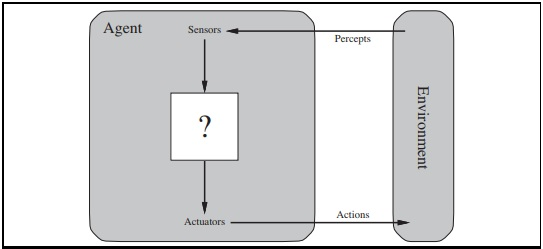
\includegraphics[width=0.6\textwidth]{image/Figura1}
\end{center}
\begin{center}
\vskip -0.5cm
\caption{\small{Estructura básica de un agente.}}
{\small{Fuente: \cite{Russel}}}
\end{center}
\end{figure}


\subsection{Caracteristicas}
Las principales características que podemos observar que  posee un agente inteligente se presentan a continuación:

\begin{enumerate}
\item[•] {\bf Autonomía:} Los agentes deben trabajar sin supervisión humana, al contrario que los programas que operan en base a interfaces de manipulación directa por parte del usuario. Así, una vez fijadas las condiciones y restricciones necesarias por parte del usuario, se espera que el agente intente cubrir o conseguir sus objetivos, dejando ocultos los detalles para dicho usuario \citep{Michael}.
\item[•] {\bf Reactividad:} los agentes deben ser capaces de detectar cambios en su entorno y en consecuencia tomar sus propias decisiones para reaccionar ante ellos.
\item[•] {\bf Adaptabilidad:} Dado a que los agentes reaccionan a los cambios producidos por el entorno, estos provocan que los agentes continuamente aprendan de estas experiencias y se adapten a dichos cambios.
\item[•] {\bf Comunicación:} El agente tiene que tener la capacidad de comunicarse por medio de un lenguaje común con otros agentes de su medio y con los usuarios que interactúa.

\item[•] {\bf Comunicación:} El agente tiene que tener la capacidad de comunicarse por medio de un lenguaje común con otros agentes de su medio y con los usuarios que interactúa.

\end{enumerate}


\section{Sustentabilidad}

{\bf Ejemplo:}\par

La configuración, característica, jurisdicción administrativa, relaciones económicas, sociales y ambientales de un espacio urbano se define por la población y por la función que ella desarrolla en un área geográfica o región \citep{Bugliarello}. De este modo las ciudades son sistemas dinámicos que interactúan continua y constantemente con su medio ambiente, acompañando las características, perfil, cultura y ritmo de desarrollo económico y social de su población. Los medios de transporte juegan un papel importante en tal ritmo de desarrollo de las ciudades, ya que ellos tienen como función relacional los factores poblacionales con los factores uso del suelo.  
\vskip 1cm
El desarrollo sustentable, (Figura 2.1), estará garantizado si se consideran tres aspectos fundamentales: económico, social y ambiental, donde la intersección de estos aspectos garantiza la calidad de vida en el espacio urbano y el equilibrio en las clases sociales en busca del bienestar \citep{Tanguay}.

\begin{figure}[ht]
\begin{center}
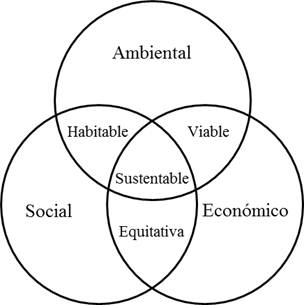
\includegraphics[width=0.3\textwidth]{image/Figura2}
\end{center}
\begin{center}
\vskip -0.5cm
\caption{\small{Aspectos claves para el desarrollo sustentable.}}
{\small{Fuente: \cite{Tanguay}}}
\end{center}
\end{figure}

\section{Logística directa y reversa}

\subsection{Logística directa}

{\bf Ejemplo:}\par

\cite{Ghiani} entienden que la logística trata de la planificación y control de los flujos de materiales e informaciones relacionadas en las organizaciones, tanto en los sectores público y privado. Además su misión es hacer la entrega de los productos correctos, en el local correcto y en la hora correcta, optimizando los costos operacionales totales del proceso.
satisfaciendo un determinado conjunto de restricciones o condiciones.\par

\subsection{Logística reversa}

{\bf Ejemplo:}\par

En los años 90 se presentaron definiciones generales las cuales vienen siendo mejoradas. \cite{Dekker} presenta una mejora en la definición de logística reversa como  ”el proceso de planificación, implementación y control de los flujos de materias-primas, en procesos de inventarios y bienes acabados, desde el punto de fabricación, distribución o uso, hacia el punto de recuperación o de eliminación”. 
\begin{figure}[ht]
\begin{center}
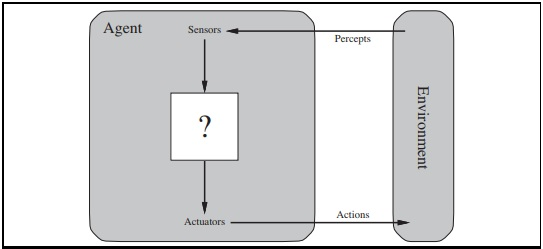
\includegraphics[width=0.3\textwidth]{image/Figura1}
\end{center}
\begin{center}
\vskip -0.5cm
\caption{\small{Logística reversa incluida en el desarrollo sustentable.}}
{\small{Fuente: Adaptación de \cite{Tanguay}}}
\end{center}
\end{figure}


\subsubsection{Modelos}

\section{Modelamiento y ruteo }

{\bf Ejemplo:}\par

El modelamiento matemático es una alternativa para expresar formalmente hechos reales que pueden ayudar en el proceso de toma de decisiones. El modelamiento permite la simulación de procesos  y de escenarios con la introducción de índices de desempeño que permitan cuantificar los costos y beneficios de la implementación del sistema, la mejoría de la sustentabilidad urbana y por supuesto los índices de contaminación en las grandes ciudades y su impacto en todo el medio ambiente. 

\subsection{Modelos utilizados en los problemas de ruteo de vehículo }

{\bf Ejemplo:}\par

El problema de ruteo de vehículos \citep{Ombuki, Yeun} y sus variantes han ganado mucho interés en la comunidad académica. La intención de estar más cerca a la realidad mediante el modelamiento matemático, hace que se hayan desarrollado nuevos modelos de optimización. \par
\vskip 0.3cm
Según \cite{Sterle} el primer nivel de la red comprende la distribución de la carga desde las plataformas hasta las unidades satélites, utilizando vehículos de carga de mayor tamaño (g).  El segundo nivel, consiste en montar rutas desde las unidades satélites hasta los clientes, usando para este caso vehículos de menor tamaño (v). El modelo de localización y ruteo de vehículos para la distribución de carga propuesto por el autor, además de hacer la conexión de los dos niveles y estudiar su inter relación y dependencia, el modelo busca determinar la cantidad necesaria de plataforma y de unidades satélites considerando el tamaño y dimensionamiento de la flota para el ruteo en dos niveles. 
\vskip 0.2cm

\begin{table}[h!]
\begin{center}
\caption{\small{Resultados computacionales obtenidos en el modelo de \cite{Sterle}}}
\end{center}
\vskip -0.7cm
\begin{tabular}{|c|c|c|c|c|}
\hline 
\rowcolor{LightBlue2}{\small Escenarios} & {\small Demanda cliente (ton.)} & {\small Tiempo (min.)} & {\small Costo ($\$$)} \\ 
\hline 
{\small 1} & {\small P1:1; P2:2; P3:2; P4:2; P5:1} & {\small 0.12} & {\small 667.42} \\ 
\hline 
{\small 2} & {\small P1:1; P2:2; P3:2; P4:2; P5:1; P:4; P7:3} & {\small 56.54} & {\small 1744.35} \\ 
\hline 
{\small 3} & {\small P1: 1; P2:2; P3:2; P4:2; P5:1; P6: 4; P7:3; P8:2; P9:2} & {\small 287.70} & {\small 1750.72} \\ 
\hline 
{\small 4} & {\small P1:1; P2:2; P3: 2; P4:2; P5:1; P6:4; P7:3; P8:2; P9:2; P10:1} & {\small 1848.57} & {\small 1773.46} \\ 
\hline 
{\small 5} & {\small P1:1; P2:2; P3: 2; P4:2; P5:1; P6:4; P7:3; P8:2; P9:2; P10:1} & {\small 1848.57} & {\small 1773.46} \\ 
\hline 
{\small 6} & {\small P1:1; P2:2; P3: 2; P4:2; P5:1; P6:4; P7:3; P8:2; P9:2; P10:1} & {\small 1848.57} & {\small 1773.46} \\ 
\hline 
\end{tabular} 
\begin{center}
\vskip -0.2cm
{\small{Fuente: Resultados obtenidos con CPLEX.}}
\end{center}
\end{table}





\chapter{Nombre de la propuesta o tema central de la tesis}

{\bf Ejemplo:}\par

Basado en los conceptos discutidos en los capítulos 1 y 2, así como de la experiencia obtenida del análisis de resultados de los modelos matemáticos estudiados y programados con CPLEX, se caracterizan los principales elementos que componen el modelo propuesto en este trabajo para la colecta y transporte de RSU en un área urbana. Así, se estructura una red logística reversa para los RSU considerando diferentes centros especializados o unidades  productivas para atender las diferentes fases del proceso en la red. En este proceso de modelamiento se tuvo cuidado en mantener la propuesta lo mas cerca a la realidad de las ciudades, donde el modelo fue testado y validado.

\section{Proceso de modelamiento} 

{\bf Ejemplo:}\par

La planificación y modelamiento del sistema de logística reversa de una área urbana es una fase importante y estratégica, para obtener en el futuro óptimos resultados en el proceso de gerenciamiento y operación del sistema reverso de RSU. El modelamiento permite determinar la localización de las estaciones de colecta y de unidades especiales necesarias, asi como el flujo que será movido a los largo de la red permitiendo dimensionar todo el sistema y sus componentes (Figura 3.1).
\vskip 0.3cm
\begin{figure}[ht]
\begin{center}
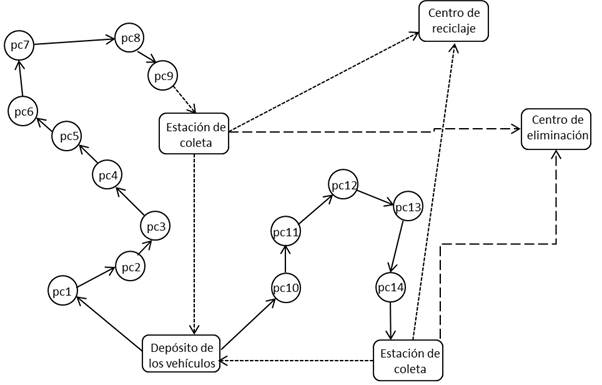
\includegraphics[width=.6\textwidth]{image/Figura3}
\end{center}
\begin{center}
\vskip -0.5cm
\caption{\small{Esquema del proceso de colecta y transporte de RSU.}}
{\small{Fuente: Elaboración propia}}
\end{center}
\end{figure}

\subsection{Proceso de ruteo}



\chapter{Resultados de la tesis}


Al culminar con la investigación se llegaron a resultados interesantes del punto de vista tanto teórico como computacional. Estos resultados muestran que se contrasta la hipótesis planteada durante el proceso de elaboración del plan de investigación, es decir, que se logró demostrar la relación entre las variables de estudio formuladas en la investigación.

\section{Teóricos}
\section{Computacionales}




\chapter{Consideraciones finales}



\section{Conclusiones}

{\bf Ejemplo}\\
La investigación bibliográfica revela que realmente existe una preocupación de los gobiernos federales con el destino final de los residuos sólidos, con el objetivo de preservar la salud de la población y el medio ambiente urbano y rural. Por ejemplo, se observa la creación, en el caso del Brasil, de la Ley 12.305/10. Sin embargo existe una laguna entre las metas propuestas en la ley con las metas reales de los gobiernos locales. Eso se debe a la falta de una buena estructura organizacional, gerencial y operacional de los gobiernos locales capaz de atender las demandas locales y las necesidades de la población.
\vskip 0.3cm
La falta de cuadros especializados, tanto en los gobiernos centrales como locales, para realizar la planificación y modelamiento de una red logística reversa puede ser compensada con la contribución de los investigadores que actúan en ese campo del conocimiento. Es muy difícil la formación de un equipo que tenga todo el conocimiento en las áreas de ciencia de la computación, de geo procesamiento, de modelamiento matemático y de logística reversa, entre otras. Esa es una de las principales justificativas que los gobiernos, federales y locales, argumentan a la falta de planificación de una red logística reversa que funciones eficaz y eficientemente. 
\vskip 0.3cm
Por lo tanto, como quedó demostrado a lo largo de este trabajo, es posible realizar el modelamiento matemático para este tipo de problema con baja inversión, así como aplicarlo en varias regiones sin necesidad de grandes cambios en el modelamiento propuesto. El modelo propuesto calcula los flujos en la red logística reversa, permitiendo dimensionar la cantidad y capacidad de las unidades productivas y de los vehículos. 
\vskip 0.3cm
...


\section{Trabajos futuros}



